
%==============================================================================
% Voorbeeld gebruik documentklasse hogent-article
%==============================================================================
%
% Compileren in TeXstudio:
%
% - Zorg dat Biber de bibliografie compileert (en niet Biblatex)
%   Options > Configure > Build > Default Bibliography Tool: "txs:///biber"
% - F5 om te compileren en het resultaat te bekijken.
% - Als de bibliografie niet zichtbaar is, probeer dan F5 - F8 - F5
%   Met F8 compileer je de bibliografie apart.
%
% Als je JabRef gebruikt voor het bijhouden van de bibliografie, zorg dan
% dat je in ``biblatex''-modus opslaat: File > Switch to BibLaTeX mode.

\documentclass{hogent-article}

%images
\usepackage{graphicx}
\graphicspath{ {./img/} }

%------------------------------------------------------------------------------
% Metadata over het artikel
%------------------------------------------------------------------------------

%---------- Titel & auteur ----------------------------------------------------
\PaperTitle{Heeft de factor muziek invloed op de resultaten van de retrieval practice studiemethode?}
% Dit is typisch de opdracht en het vak waarvoor dit artikel geschreven is, bv.
% ``Verslag onderzoeksproject Onderzoekstechnieken 2018-2019''
\PaperType{Verslag onderzoeksproject Onderzoekstechnieken 2018-2019}

\Authors{Olivier Troch\textsuperscript{1}, Daan Van Vooren \textsuperscript{2}, Robbie Verdurme\textsuperscript{3}, Sebastien Wojtyla\textsuperscript{4}} % Authors



% Als het hier gaat om een voorstel voor de bachelorproef, dan ben je hier
% verplicht de naam van je co-promotor in te vullen. Zoniet, dan kan je het
% leeg laten.
\CoPromotor{}

% Contactinfo: Geef hier de contactgegevens van elke auteur van het artikel (en
% indien van toepassing ook van de co-promotor).
\affiliation{
	\textsuperscript{1} \href{mailto:Olivier.troch.w2257@student.hogent.be}{Olivier.troch.w2257@student.hogent.be}
}
\affiliation{
	\textsuperscript{2} \href{mailto:daan.vanvooren.y1502@student.hogent.be}{daan.vanvooren.y1502@student.hogent.be}
}
\affiliation{
	\textsuperscript{3}
	\href{mailto:robbie.verdurme.y9234@student.hogent.be}{robbie.verdurme.y9234@student.hogent.be}
}
\affiliation{
	\textsuperscript{4}
	\href{mailto;sebastien.wojtyla.y3274@student.hogent.be}{sebastien.wojtyla.y3274@student.hogent.be}
}
%---------- Abstract ----------------------------------------------------------
\Abstract{In deze paper wordt onderzocht wat de effecten zijn op de resultaten van de retrieval practice studiemethode.
	In veel studies werd reeds aangetoond dat retrieval practice een goede studiemethode is maar welke factoren hierop invloed hebben is minder besproken. De paper gaat dieper in op deze vraag door te onderzoeken of het beluisteren van muziek gedurende de retrieval practice methode enige invloed zal hebben op de resultaten.
	De te verwachte resultaten zijn dat het beluisteren van muziek tijdens de retrieval practice studiemethode een negatief effect zullen hebben. Deze paper kan bijdragen aan verder onderzoek van de retrieval practice methode.
}

%---------- Onderzoeksdomein en sleutelwoorden --------------------------------
\Keywords{Onderzoeksproces, Studiemethodes, Retrieval Practice}
\newcommand{\keywordname}{Sleutelwoorden} % Defines the keywords heading name

%---------- Titel, inhoud -----------------------------------------------------

\begin{document}
	
	\flushbottom % Makes all text pages the same height
	\maketitle % Print the title and abstract box
	\tableofcontents % Print the contents section
	\thispagestyle{empty} % Removes page numbering from the first page
	
	%------------------------------------------------------------------------------
	% Hoofdtekst
	%------------------------------------------------------------------------------
	
	\section{Inleiding}
	Retrieval practice is een studiemethode die ervoor zorgt dat leerstof langer onthouden kan worden op lange termijn. Hoewel reeds aangetoond is dat dit een effectieve methode is voor het studeren verwachten wij een ander resultaat wanneer we een variabele aanpassen. De variable die we zullen testen in deze paper is het effect van muziek tijdens het instuderen van een tekst.
	
	
	\section{Overzicht literatuur}
	
	% Refereren naar de literatuur kan met:
	% \autocite{BIBTEXKEY} -> (Auteur, jaartal)
	% \textcite{BIBTEXKEY} -> Auteur (jaartal)
	% Voorbeeld van een referentie~\autocite{Moore2002}
	
	
	
	\section{Methodologie}
	De variabele die getest word in deze paper is het effect van muziek beluisteren tijdens de retrieval practice methode.
	Door het beluisteren van muziek tijdens het instuderen kan het brein meer gestimuleerd worden. Hierdoor zal het brein ook de studiematerie kunnen linken aan de geluisterdde liederen en zo gemakkelijker de nieuwe materie kan onthouden.
	Dit kan een grote invloed hebben op het studeren zoals reeds bewezen is \autocite{ChanEtAl1998}.
	


	
	\section{Experimenten}
	Tijdens het onderzoek krijgt iedere informatica student een tekst over darwin die hij/zij zal moeten bestuderen. Vervolgens wordt de groep opgesplitst in vier subgroepen. Elke subgroep zal de standaard retrieval practice methode (STST) toepassen waarvan twee subgroepen met een aangepaste variabele.
	De eerste subgroep zal de standaard retrieval practice methode toepassen zonder aangepaste variabele. 

	De tweede subgroep zal muziek te horen krijgen tijdens het instuderen van de tekst. In combinatie met deze variable muziek zal er nog altijd gewerkt worden met de Retrieval practice
	
	De derde subgroep zal muziek te horen krijgen tijdens het instuderen van de tekst maar doet dit niet aan de hand van de Retrieval practice methode
	
	De vierde groep zal geen muziek te horen krijgen tijdens het instuderen van de tekst en zal ook niet te werk gaan aan de hand van de Retrieval practice methode
	
	Hierdoor kan nagegaan worden of de variabelen een invloed hebben op het studeren van een tekst aan de hand van de retrieval practice methode. Merk op dat we elke tweedejaars informatica student er toe verplichten om deel te nemen aan deze test waardoor het resultaat niet op de hele groep studenten toepasbaar is zonder enig foutpercentage \autocite{karpicke2009metacognitive}.
	
	\section{Verwactingen}
	We veronderstellen dat de eerste subgroep analoge resultaten zal behalen aan de resultaten uit de artikels over de retrieval practice methode \autocite{butler2010repeated, pyc2012test, karpicke2007repeated, karpicke2008critical}. Dit is omdat deze methode reeds vaak getest werd in verschillende experimenten.
	
	Daarnaast verwachten we dat het beluisteren van muziek een negatief effect zal hebben op het resultaat. Door het beluisteren van muziek kan je sneller afgeleid graken tijdens het lezen van de tekst en deze dan ook minder gemakkelijk onthouden.
	
	\section{Analyse resultaten}
	\subsection{Retrieval Practice}	
	%met rt en zonder rt vergelijken
	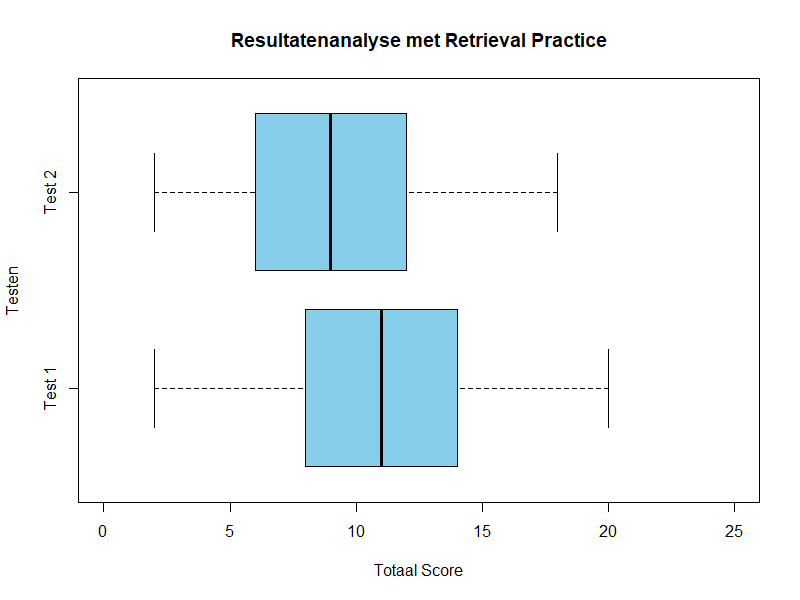
\includegraphics[width=50px]{Rplot_MetRetrievalPractice}
	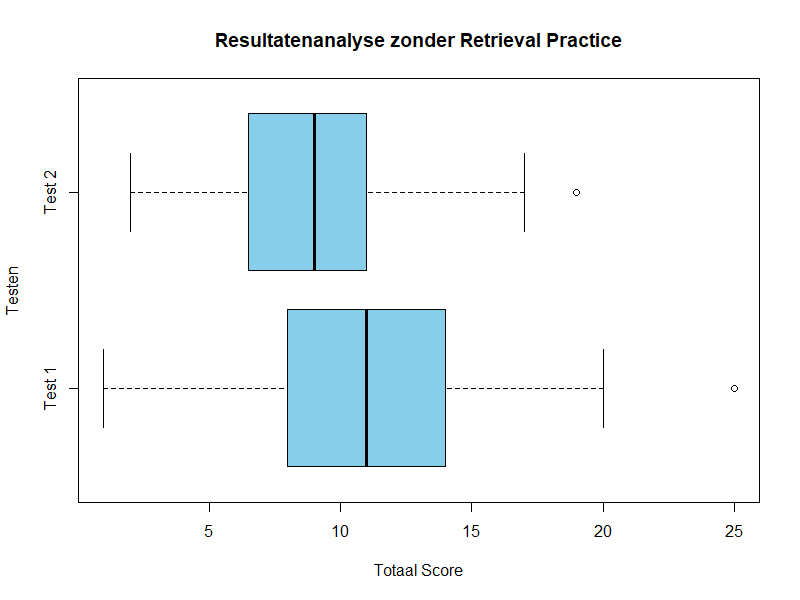
\includegraphics[width=50px]{Rplot_ZonderRetrievalPractice}
	
	\subsection{Muziek}
	%met muziek en zonder muziek vergelijken
	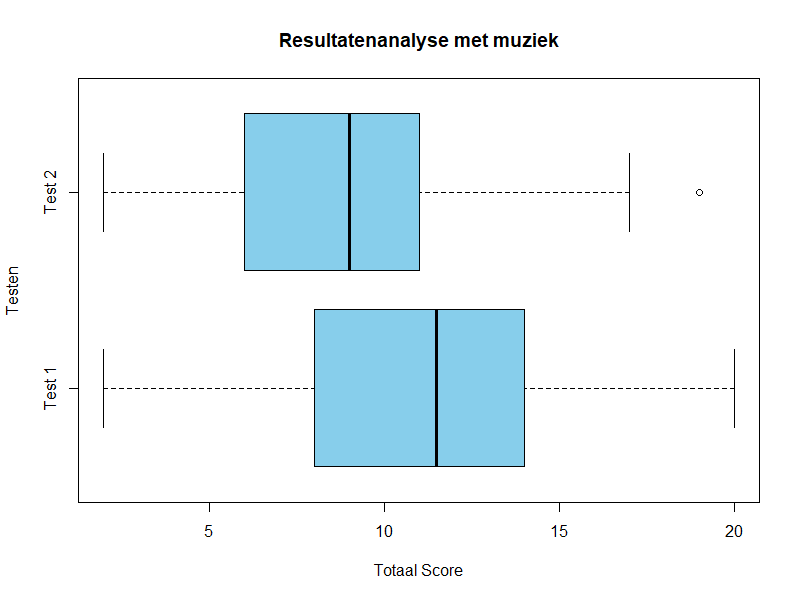
\includegraphics[width=50px]{Rplot_MetMuziek}	
	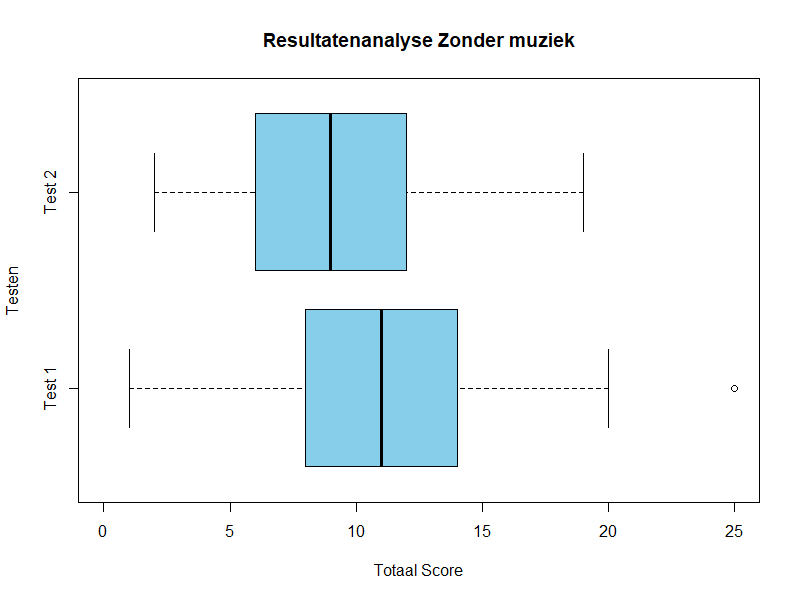
\includegraphics[width=50px]{Rplot_ZonderMuziek}
		
	
	\subsection{Retieval Practice met Muziek}
	%met rt en muziek vergelijken
	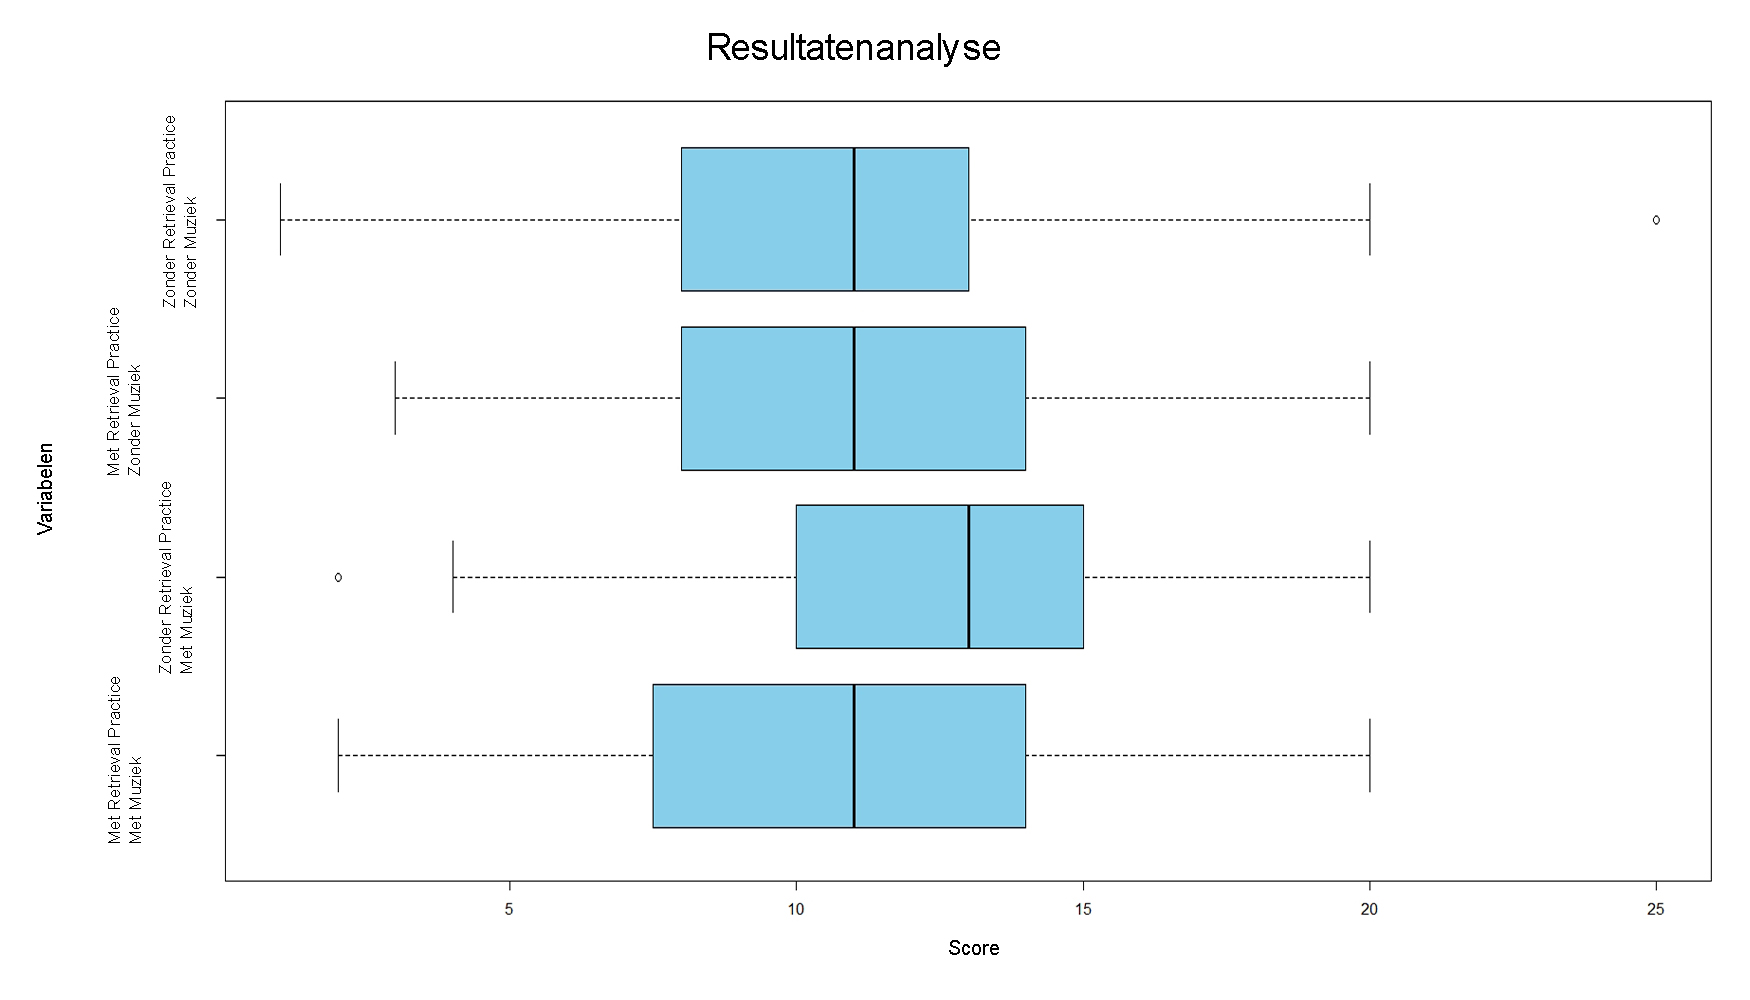
\includegraphics[width=50px]{Rplot_RetrievalPracticeMuziek_Score1}	
	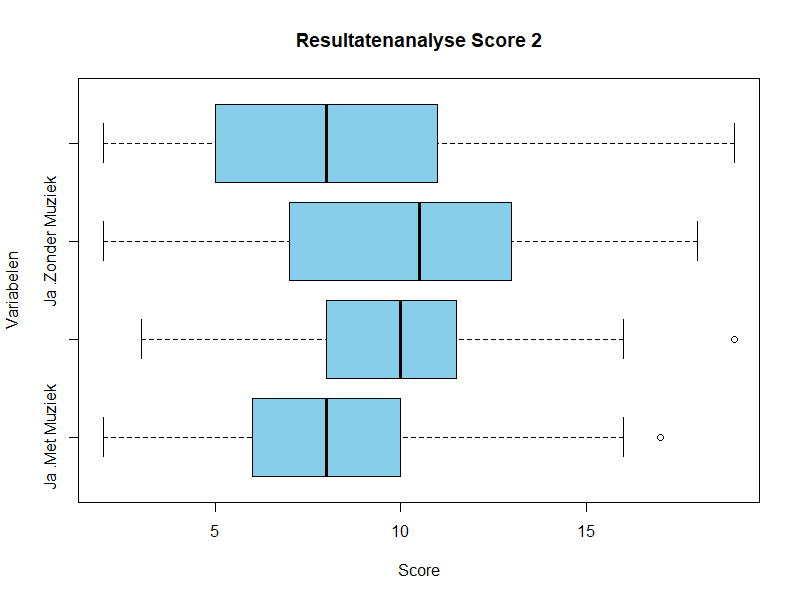
\includegraphics[width=50px]{Rplot_RetrievalPracticeMuziek_Score2}
	
	
	
	%%EXTRA BOXPLOTS
		%%met en zonder muziek per test
%		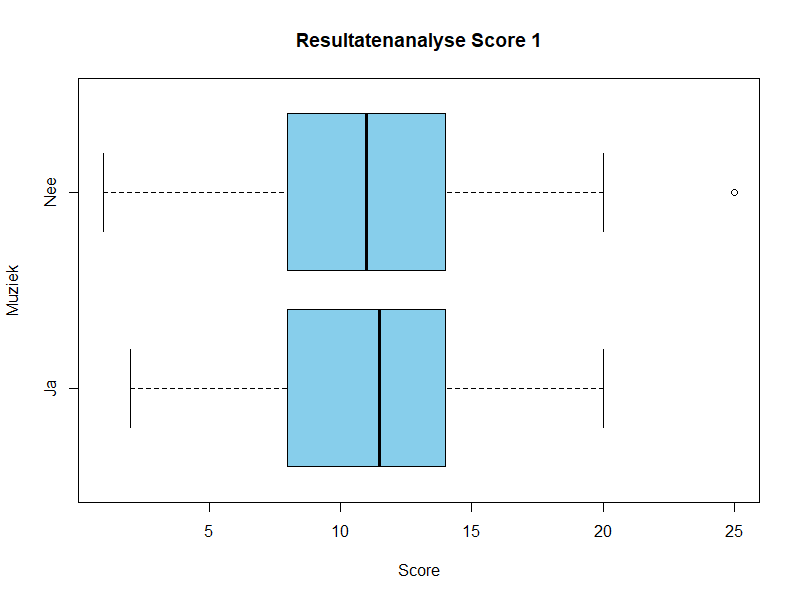
\includegraphics[width=50px]{Rplot_Muziek_Score1}
%		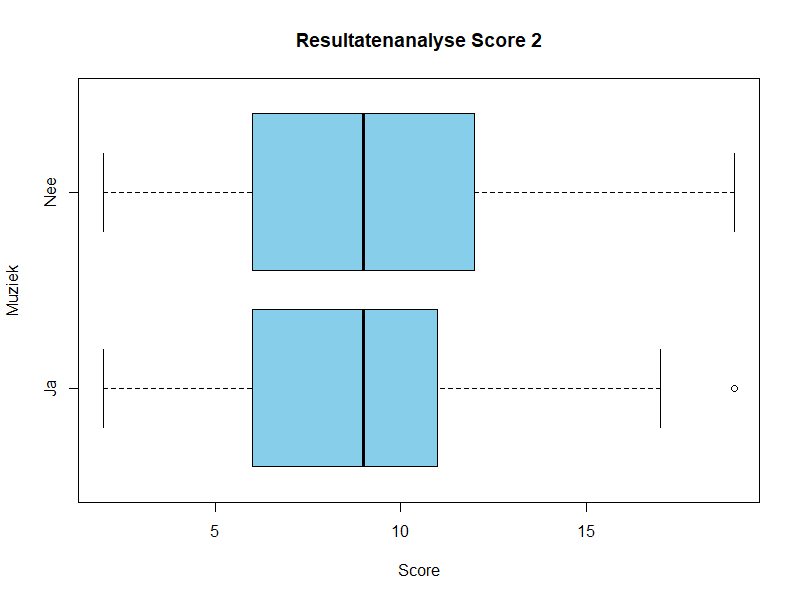
\includegraphics[width=50px]{Rplot_Muziek_Score2}
		%% met zonder retrieval practice per test
%		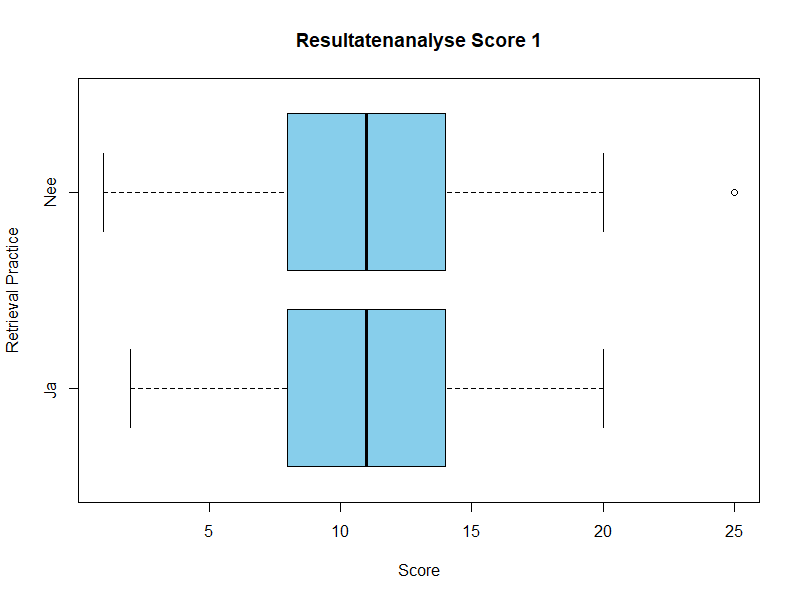
\includegraphics[width=50px]{Rplot_RetrievalPractice_Score1}
%		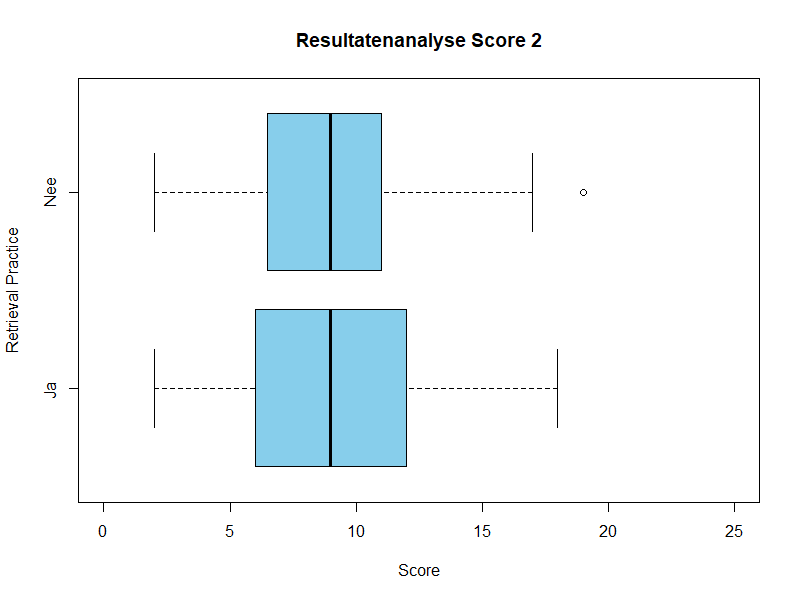
\includegraphics[width=50px]{Rplot_RetrievalPractice_Score2}
	\section{Conclusie}
	
	
	
	%------------------------------------------------------------------------------
	% Referentielijst
	%------------------------------------------------------------------------------
	% voorkomen. Gebruik JabRef om je bibliografie bij te houden en vergeet niet
	% om compatibiliteit met Biber/BibLaTeX aan te zetten (File > Switch to
	% BibLaTeX mode)
	
	\phantomsection
	\printbibliography[heading=bibintoc]
	
\end{document}
